\documentclass[a4paper,11pt,twoside]{report}
\usepackage[T1]{fontenc}
\usepackage[frenchb]{babel} %active le mode français
\usepackage[latin1,utf8]{inputenc} % Mettre des accents
\usepackage[top=2cm , bottom=2cm , left=2cm , right=2cm]{geometry} %propriétés de notre page
\usepackage{amsmath} %liste de symboles et applications mathématiques
\usepackage{amsfonts} %idem
\usepackage{color} %Permet d'utiliser la couleur dans nos documents
\usepackage[usenames,dvipsnames]{xcolor}
\usepackage{listings} %Paquet de coloration syntaxique (langages)
\usepackage{hyperref} % Créer des liens et des signets 
\usepackage[babel=true]{csquotes} %permet les quotations (guillemets)
\usepackage{graphicx} %Importation d'image
\usepackage{fancyhdr} %en-tête et pieds de page+
\usepackage{lastpage} %permet d'obtenir le nombre total de page
\usepackage{multido}
\usepackage{eurosym}
\usepackage{listingsutf8}
\usepackage{tikz}
\usepackage{ulem}
\usepackage{colortbl} %permet de mettre de personnaliser les colones des tabular
\usepackage{pdfpages}
\setlength{\headheight}{15pt}
\lstset{language=C,
	breaklines=true,
	numbers=left,
	keywordstyle=\color{blue},
	commentstyle=\color{Gray},
	stringstyle=\color{red},
	tabsize=4,
	framexleftmargin=7mm,
	frame=single
	}
% Informations du rapport
\title {Rapport de projet \\ Le Problème PLTC}
\author {Quentin Tonneau - Adrien Lardenois}
\date{}
%Propriétés des liens
% \hypersetup{
% colorlinks=true, %colorise les liens  
% urlcolor= blue, %couleur des hyperliens 
% linkcolor= blue,%couleur des liens internes
% citecolor=black
% } 
%\setlength{\parindent}{0cm}
\addto\captionsfrench{
	\renewcommand{\chaptername}{Partie}
}

\fancypagestyle{plain}
{

	\fancyhead{}
	\fancyfoot{}
	\lhead{Quentin Tonneau - Adrien Lardenois}
	\rhead{Université de Nantes}
	\chead{Le problème PTLC}
}
\begin{document}
\pagestyle{plain}
\renewcommand\labelitemi{$\circ$}
\renewcommand\labelitemii{$\bullet$}
\tableofcontents
\newpage
\thispagestyle{empty} ~

\fancypagestyle{plain}
{

	\fancyhead{}
	\fancyfoot{}
	\lhead{Quentin Tonneau - Adrien Lardenois}
	\rhead{Université de Nantes}
	\chead{Recherche topswops}
	\lfoot[\thepage]{}
	\rfoot[]{\thepage}
}

\part{Introduction}
 
\part{Les algorithmes}
\section{Choix d'impl�mentation}
  
  Nous avons choisi d'impl�menter ces algorithmes en C++, � la fois simple � aborder et efficace.
  
  \subsection{Algorithme 1}
  Pour implementer l'algorithme 1, nous avons choisi de repr�senter Mlsuff comme un int**.\\
  
  Le remplissage de la matrice se fait en deux temps : \begin{itemize}
  \item On remplit la premiere ligne et la premiere colonne de la matrice, qui revient � comparer le premier caract�re de chaque tableau avec chacun de ceux de l'autre tableau.
  \item On remplit le reste du tableau gr�ce � la formule liant Mlsuff\[i\]\[j\] � Mlsuff\[i+1\]\[j+1\].
  \end{itemize}
  \vspace{0.5cm}
  
  on reparcourt ensuite chaque case du tableau pour conserver le maximum que l'on renvoie en fin de parcours.\\
  
  \subsection{Algorithme 2}
  
	Cet algorithme est impl�ment� par 3 boucles \textbf{for} imbriqu�es : \begin{itemize}
\item Une pour traiter toutes les tailles de 1 � n.
\item Une pour choisir chaque sous-cha�ne de la taille en cours dans S.
\item Une pour choisir chaque sous-cha�ne de la taille en cours dans T.
 \end{itemize}
 \vspace{0.5cm}
 
 Au sein de la derniere boucle, on effectue la comparaison de la paire de cha�ne en cours et si la condition est respect�e on affecte la nouvelle valeur � {\textbf max}.
 
  \subsection{Algorithme 3}
	
	Cet algorithme est principalement cod� comme une boucle {\textbf tant que} pour le remplissage d'un tableau PMK (int*), et d'une boucle {\textbf for} pour la comparaison avec T.\\
	
	Ces �tapes sont �x�cut�es syst�matiquement au sein de 2 boucles {\textbf for}.\\
	
	Le tableau $S_{ij}$ n'est jamais cr��, on se contente d'acceder � la case de S en op�rant un d�calage en fonction du i et du j actuel. On �vite ainsi de cr�er et recopier le tableau pour chaque paire de i j.
	
\section{Complexit� th�orique}
  \subsection{Algorithme 1}
  l'algorithme n�cessite de parcourir 2 fois une matrice de taille n par n, ce qui �quivaut � une complexit� en $O(n^2)$ pour les parcours.\\

  Les m�mes op�rations sont effectu�es sur chaque case, elles sont donc ind�pendantes de n, ce sont des op�rations d'affectation, de test d'�galit� et d'addition, c'est � dire toutes en $O(1)$.\\

  La complexit� reste donc en $O(n^2)$.
  
  \subsection{Algorithme 2}
	Cet algorithme contient 3 boucles imbriqu�es dont la longueur d�pend de la taille n des donn�es (sans �tre �gale � n).\\
	
	A l'interieur de ces boucles, on effectue la comparaison de deux cha�nes de taille l ( $1 \leq l \leq n$ ), ce qui donne une op�ration de complexit� $O(l)$, soit au pire $O(n)$.\\
	
	Nous obtenons donc une complexit� en $O(n^4)$
	
	
  \subsection{Algorithme 3}
  
	L'algorithme s'ex�cute pour toute paire i,j avec ($ 1 \leq i \leq j \leq n$). Cela revient � une boucle de complexit� $O(n^2)$.\\

	La premi�re partie de l'algorithme est une boucle {\textbf tant que}, {\textbf a} augmentant r�guli�rement et {\textbf sij } allant de 1 � n, on obtient une complexit� $O(n)$ pour cette boucle. De plus tout ce que s'effectue au sein de la boucle est en $O(1)$ y compris la boucle des lignes 6-8.\\

	La seconde partie est une boucle {\textbf Pour } de taille n. De m�me tout ce qui s'effectue � l'interieur est en $O(1)$.\\
	
	Le nombre d'op�rations n�cessaires est donc en $O(n)$ au sein d'une boucle en $O(n^2)$.
	
	On a donc une complexit� globale en $O(n^3)$.
	

 
\part{Méthode d'analyse}
   \section{Génération exhaustive}
      Afin de générer l'ensemble des chaînes possibles de taille n pour un alphabet $\{A,B,C,D\}$, nous avons eu recours à un script en langage \textbf{prolog} (voir Annexe \ref{code_prolog}).
Ce langage permet de facilement écrire des scripts usant (et abusant) du backtracking. Le script choisi une lettre à la position $i$ ($i\in \{1..n\})$, créé un point de choix, et passe à la case suivante.
Une fois le mot formé, l'algorithme effectue un backtrack sur ses points de choix et génère ainsi l'ensemble des chaînes possibles. On utilise la redirection de sortie standard (commande \textit{>} en shell linux) de ce programme vers un fichier.
On obtient par exemple sur une taille $n=2$ le fichier suivant :\\
\begin{center}
 \fbox{
\begin{minipage}{0.9\textwidth}\centering
 2
AA
AT
AC
AG
TA
TT
TC
TG
CA
CT
CC
CG
GA
GT
GC
GG
\end{minipage}
}
\end{center}

Comparer toutes les chaînes générées, nous simulons la présence de deux curseurs dans le fichier, le premier parcourant les chaînes S, et le second toutes les suivantes (T).
   \section{Génération aléatoire}
      Afin de générer aléatoirement des chaînes de taille $n$, nous créons la fonction \textit{random\_generate}, qui comme son nom l'indique, se repose sur la fonction rand() du langage C++ :

\begin{center}
\begin{minipage}{0.9\textwidth}
\begin{center}
\begin{lstlisting}
  //Generate a random ADM sequence (size = n)
// O(n) - Need to free the result
char* random_generate(const int &n,int randomvalue)
{
  srand(time(NULL)+randomvalue);
  char ADN[4]={'A','T','C','G'};
  char* result=(char*) malloc((n+2)*sizeof(char));
  int i;
  result[0]='x';
  for(i=0;i<n;i++)
  {
    result[i+1]=ADN[rand()%4];
  }
  result[i+1]='\0';
  return result;
}
\end{lstlisting}
\end{center}
\end{minipage} 
\end{center}

La présence de l'entier \textbf{randomvalue} réside dans le fait que la fonction random n'est pas totalement aléaoire, et dépend en partie de l'heure système (en seconde).
Ainsi, en appelant plusieurs fois la fonction dans la même seconde, les chaînes retournées seront toujours identiques. Il faut donc penser à incrémenter le compteur à chaque génération, et conserver la base de temps initial\footnote{À voir dans l'algorithme principal}.

   \section{Algorithme principal}
      L'algorithme principal est en charge de génèrer ou de charger un ensemble de jeux de test selon la demande de l'utilisateur. Le programme doit être appelé selon la commande suivante :\\
\begin{verbatim}
 <executable> <numero de l'algorithme> [{<taille>|<fichier d'instance>}]*
\end{verbatim}

Ce dernier récupère donc en premier argument le numéro (1,2,3) de l'algorithme sélectionné, et génère un nombre de jeux de test aléatoire dans un temps inférieur à 3 minutes si le paramètre est un chiffre, ou récupère et ``appaire'' toutes les chaînes du fichier dont le nom correspond à ce paramètre\footnote{De ce fait, les noms de fichier ne doivent pas commencer par un chiffre}.\\
Ensuite, une fonction de chronométrage se lance au début de la comparaison de deux chaînes, et s'arrête à la fin de celle-ci. Un ensemble de variables (min, max, time, sum) s'occupe de conserver et gérer les statistiques temporelles liées à ces exécutions.


Nous avons choisi cette implémentation car elle permet de rester souple (si besoin de tests spécifiques, il suffit de générer par quelconque moyen un fichier correspondant), et autonome, dans la mesure ou une seule exécution permet de récupérer les résultats complets d'un algorithme (ne nécessite pas une présence sur la machine toutes les 3 minutes).

   \section{Les contraintes matérielles}
      Nous avons été confrontés à un certain nombre de problèmes lors des premiers tests. En effet, le temps d’ exécution des trois algorithmes pour des petites valeurs (inférieures à 800 caractères) se situait en dessous de la milliseconde, plus petite unité admissible dans nos algorithmes et dans le projet en général.
Afin de donner un peut plus de cohérence dans nos résultats (principalement les 12 premières lignes des tableaux), nous avons implémenté un système de boucle calculant un facteur d'exécution pour chaque jeu de test, permettant de passer outre ces limitations.
En d'autres termes, pour les petites valeurs de $n$, il est nécessaire de comparer $facteur$ fois les mêmes chaînes entre le lancement et l'arrêt du chronomètre. Ce facteur est calculé pour chaque jeux de test de la façon suivante :
\begin{lstlisting}
 facteur=1;
 tant que t(facteur resolutions)<5ms alors
    facteur <- facteur*10;
 fintantque
\end{lstlisting}

Nous précisons toutefois que la présentation des résultats et l'analyse effectuée ne reprend pas les résultats inférieurs à $1ms$ de façon exacte ($<1ms\ devient\ =0ms$).
\part{Résultats et Interprétation}
  \section{Résultats}
      %Nous avons effectué plusieurs séries de tests selon les critères de l'énoncé, c'est à dire :
\begin{itemize}
 \item Effectuer des tests exhaustifs jusqu'à atteindre une résolution totale supérieure à 3 minutes
 \item Effectuer ensuite des tests aléatoires jusqu'à une résolution totale supérieure à 3 minutes (quelque soit le nombre de test)
\end{itemize}
Nous avons, en revanche, lorsque la résolution nous obtenait un résultat légèrement supérieur à 3 minutes, ajouté une ligne supplémentaire dans le tableau.
\subsection{Algorithme 1}
\begin{table}[p]
{%
\begin{center}
\begin{tabular}{||p{1cm}||p{2.5cm}|p{2.5cm}|p{2.5cm}|p{2.5cm}|p{2.5cm}||}
\hline\hline
\multicolumn{6}{||c||}{Algorithme $A_1$ - Temps d'exécution}\\\hline\hline
$n$ & Nombre de & Analyse& \multicolumn{3}{c||}{Temps d'exécution}\\
& tests effectués & exhaustive ?  &Au mieux&en moyenne&au pire\\\hline\hline


1 & 10 & OUI& 0,000 ms & 0,000 ms & 0,000 ms\\\hline
2 & 136 & OUI & 0,000 ms & 0,000 ms & 0,000 ms\\\hline
4 & 32896 & OUI & 0,000 ms & 0,000 ms & 0,000 ms\\\hline
8 & 975800000 & NON & 0,000 ms & 0,000 ms & 0,000 ms\\\hline
10 & 614000000 & NON & 0,000 ms & 0,000 ms & 0,000 ms\\\hline
20 & 171270000 & NON & 0,000 ms & 0,001 ms & 0,002 ms\\\hline
40 & 40520000 & NON & 0,004 ms & 0,004 ms & 0,005 ms\\\hline
80 & 9656000 & NON & 0,012 ms & 0,019 ms & 0,024 ms\\\hline
100 & 6047000 & NON & 0,024 ms & 0,030 ms & 0,036 ms\\\hline
200 & 1438500 & NON & 0,080 ms & 0,125 ms & 0,170 ms\\\hline
400 & 351200 & NON & 0,440 ms & 0,513 ms & 0,570 ms\\\hline
800 & 86690 & NON & 1,600 ms & 2,076 ms & 2,500 ms\\\hline
1000 & 55300 & NON & 2,800 ms & 3,255 ms & 3,700 ms\\\hline
2000 & 10583 & NON & 0,000 ms & 17,009 ms & 29,000 ms\\\hline
4000 & 2800 & NON & 36,000 ms & 64,287 ms & 92,000 ms\\\hline
8000 & 721 & NON & 161,000 ms & 249,953 ms & 293,000 ms\\\hline
10000 & 464 & NON & 325,000 ms & 388,560 ms & 445,000 ms\\\hline
20000 & 117 & NON & 1448,000 ms & 1543,350 ms & 1653,000 ms\\\hline
40000 & DM & NON & DM & DM & DM\\\hline\hline
\end{tabular}
\caption{Résultats expérimentaux de l'algorithme 1}
\label{tab1}
\end{center}
}%
\end{table}
Les mesures présentée dans le tableau \ref{tab1} ont été effectuées avec le système de facteur présenté en partie \ref{facteur}.
Les faibles mesures (seulement une ligne au dessus de la seconde) nous impose une présentation des résultats en millisecondes.
On remarque que l'algorithme effectue un dépassement mémoire à partir de $n=40 000$. Si l'on considère un caractère encodé en 8 bits, la matrice générée est alors de $40000*40000$ octets, soit environ 6 Gibioctets de mémoire.
On s'apercoit néanmoins que cet algorithme est très rapide, comme en témoigne le graphique \ref{graphalgo1}
\begin{figure}[p]
  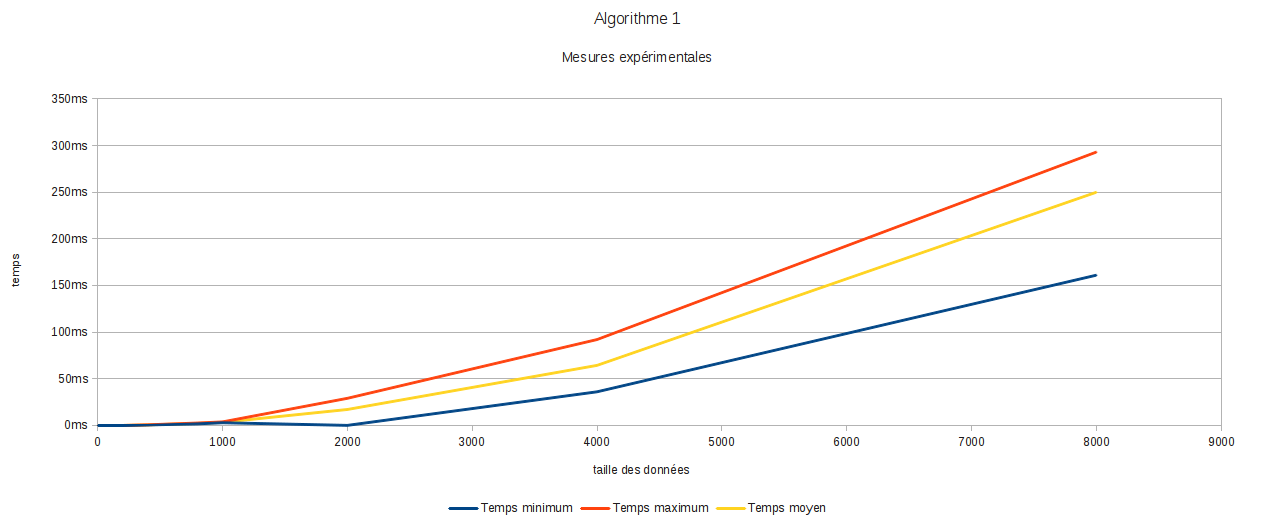
\includegraphics[width=\textwidth]{expe_algo1}
  \caption{Représentation graphique des résultats expérimentaux de l'algorithme 1}
    \label{graphalgo1}
\end{figure}

\subsection{Algorithme 2}
\begin{table}[p]
{%
\begin{center}
\begin{tabular}{||p{1cm}||p{2.5cm}|p{2.5cm}|p{2.5cm}|p{2.5cm}|p{2.5cm}||}
\hline\hline
\multicolumn{6}{||c||}{Algorithme $A_2$ - Temps d'exécution}\\\hline\hline
$n$ & Nombre de & Analyse& \multicolumn{3}{c||}{Temps d'exécution}\\
& tests effectués & exhaustive ?  &Au mieux&en moyenne&au pire\\\hline\hline

1 & 10 & OUI & 0,000 ms & 0,000 ms & 0,000 ms\\
2 & 136 & OUI & 0,000 ms & 0,000 ms & 0,000 ms\\
4 & 32896 & OUI & 0,000 ms & 0,000 ms & 0,000 ms\\
8 &  87115000 & NON & 0,001 ms & 0,002 ms & 0,004 ms\\
10 & 46420000 & NON & 0,002 ms & 0,004 ms & 0,005 ms\\
20 & 6246000 & NON & 0,016 ms & 0,029 ms & 0,040 ms\\
40 & 778800 & NON & 0,160 ms & 0,231 ms & 0,340 ms\\
80 & 93900 & NON & 1,760 ms & 1,917 ms & 2,080 ms\\
100 & 48450 & NON & 3,520 ms & 3,719 ms & 3,920 ms\\
200 & 5907 & NON & 20,000 ms & 30,474 ms & 33,000 ms\\
400 & 725 & NON & 240,000 ms & 248,346 ms & 257,000 ms\\
800 & 90 & NON & 1993,000 ms & 2014,560 ms & 2036,000 ms\\
1000 & 46 & NON & 3905,000 ms & 3931,000 ms & 3965,000 ms\\
2000 & 6 & NON & 31273,000 ms & 31313,800 ms & 31406,000 ms\\
4000 & 1 & NON & 252191,000 ms & 252191,000 ms & 252191,000 ms\\\hline\hline
\end{tabular}

\caption{Résultats expérimentaux de l'algorithme 2}

\label{tab2}
\end{center}
}%
\end{table}

La forme de l'algorithme 2 nous laisse à penser que les coûts aux pire et au mieux sont identiques. En effet, $A_2$ est constitué de trois boucles indépendantes de la forme des données, seule la taille compte. En parcourant et comparant la liste de toutes les sous-chaînes possibles, le temps d'exécution sera toujours constant, quelque soit le résultat retourné.
Les courbes confondues dans la figure \ref{graphalgo2} le prouvent. L'algorithme est toutefois plus lent que le premier, car une seule comparaison de deux chaînes de 4000 caractère prend environ 4 minutes.


\begin{figure}[p]
  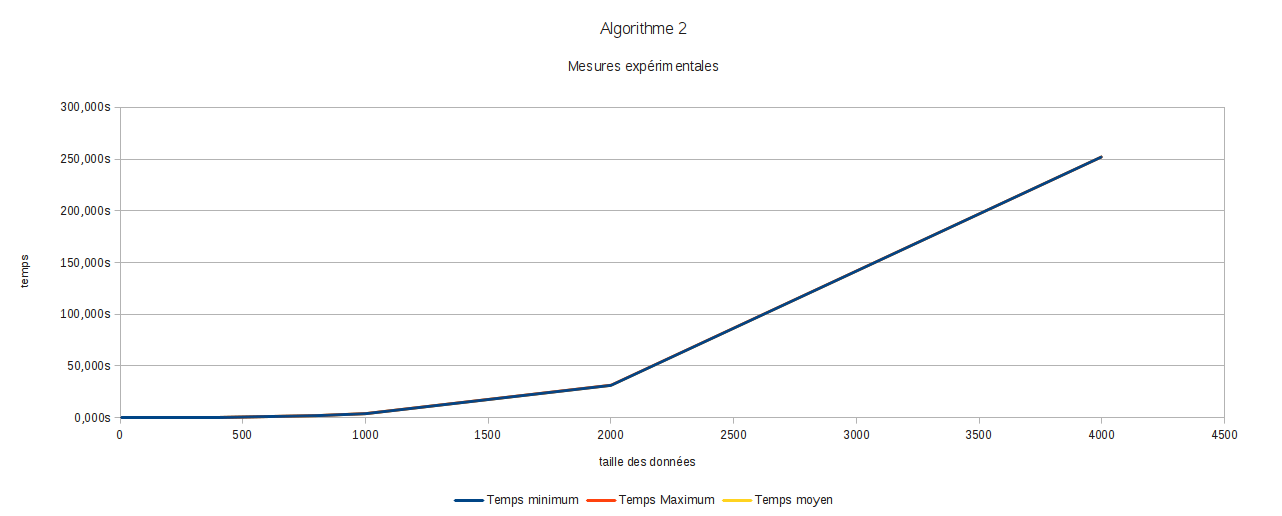
\includegraphics[width=\textwidth]{expe_algo2}
  \caption{Représentation graphique des résultats expérimentaux de l'algorithme 2}
    \label{graphalgo2}
\end{figure}

\subsection{Algorithme 3}
\begin{table}[p]
{%
\begin{center}
\begin{tabular}{||p{1cm}||p{2.5cm}|p{2.5cm}|p{2.5cm}|p{2.5cm}|p{2.5cm}||}
\hline\hline
\multicolumn{6}{||c||}{Algorithme $A_2$ - Temps d'exécution}\\\hline\hline
$n$ & Nombre de & Analyse& \multicolumn{3}{c||}{Temps d'exécution}\\
& tests effectués & exhaustive ?  &Au mieux&en moyenne&au pire\\\hline\hline

1 & 10 & NON & 0,000s & 0,000s & 0,000s\\
2 & 136 & NON & 0,000s & 0,000s & 0,000s\\
4 & 12131 & NON & 0,000s & 0,000s & 0,000s\\
8 & 43050000 & OUI & 0,000s & 0,000s & 0,000s\\
10 & 25040000 & OUI & 0,000s & 0,000s & 0,000s\\
20 & 3987800 & OUI & 0,000s & 0,000s & 0,000s\\
40 & 579700 & OUI & 0,000s & 0,000s & 0,000s\\
80 & 79300 & OUI & 0,002s & 0,002s & 0,002s\\
100 & 41190 & OUI & 0,003s & 0,004s & 0,005s\\
200 & 5276 & OUI & 0,028s & 0,034s & 0,037s\\
400 & 665 & OUI & 0,260s & 0,271s & 0,280s\\
800 & 84 & OUI & 2,136s & 2,163s & 2,200s\\
1000 & 43 & OUI & 4,200s & 4,265s & 4,329s\\
2000 & 6 & OUI & 33,727s & 33,936s & 34,134s\\
4000 & NRP & OUI & NRP & NRP & NRP\\\hline\hline
\end{tabular}

\caption{Résultats expérimentaux de l'algorithme 3}

\label{tab3}
\end{center}
}%
\end{table}
Tout comme pour l'algorithme $A_2$, les courbes de temps au mieux/au pire de l'algorithme $A_3$ sont confondues. 
Il serait pertinent de vérifier que le temps d'exécution ne dépend pas de la forme des données, mais le manque de compréhension de cet algorithme nous empêche de confirmer cette hypothèse.
\begin{figure}[p]
  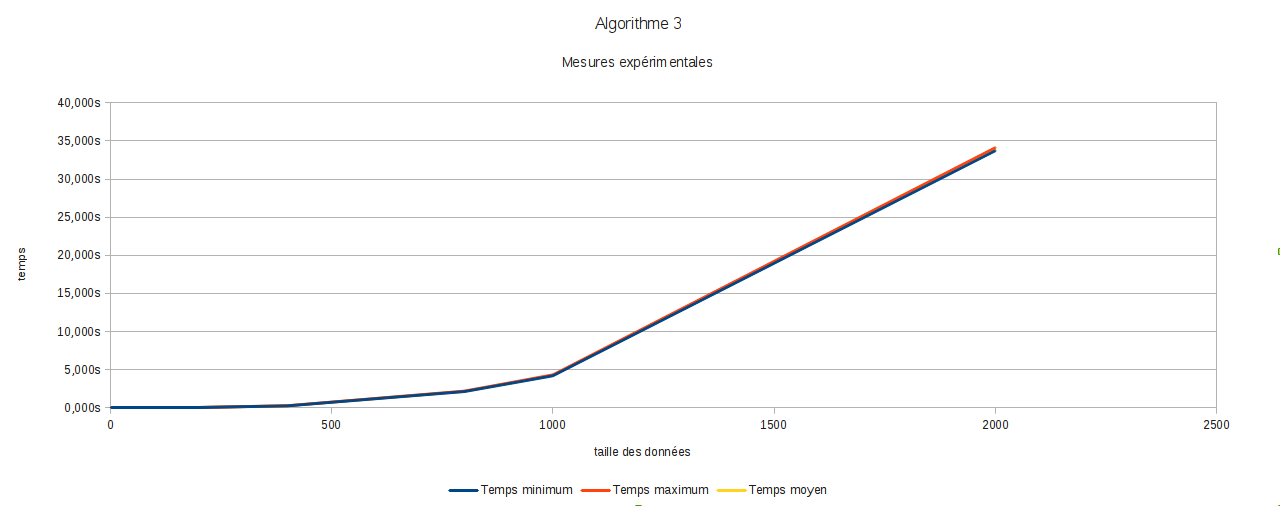
\includegraphics[width=\textwidth]{expe_algo3}
  \caption{Représentation graphique des résultats expérimentaux de l'algorithme 3}
    \label{graphalgo3}
\end{figure}
  \section{Interpolation des courbes}
      %
\subsection{Principe}
 Nous cherchons dans cette partie à exprimer une fonction passant (ou approchant) par chaque point de notre tableau expérimental. Le tableur utilisé dans ce projet (LibreOffice) ne possède pas de fonctions d'interpolation automatique pour un polynôme de degré défini.
 Nous avons alors cherché ``à la main'' cette fonction en utilisant la méthode suivante: \vspace{1cm}\\
 
 D'après l'étude théorique de la partie \ref{c_theorique}, nous connaissons le rang maximum de la fonction. Par exemple, pour l'algorithme $A_1$, nous sommes en recherche d'une forme $\alpha x^3 + \beta x^2 + \Gamma x + c$.\\
 Pour retrouver ces différents coefficients, nous avons utilisé cet algorithme :
 \begin{itemize}
  \item Augmenter $\alpha$ jusqu'à ce que les valeurs de $f(x)$ approchent des valeurs expérimentales sans les dépasser.
  \item Augmenter $\beta$ de la même manière en conservant $\alpha$ comme acquis.
  \item Réitérer pour les coefficients suivants.
 \end{itemize}
Coefficient après coefficient, nous affinons ainsi la fonction afin qu'elle approche au maximum des points connus. La pertinence de cette méthode repose essentiellement sur la qualité des mesures effectuées. En outre, si une mesure est beaucoup plus faible que la normale, notre méthode ne corrigera pas ce défaut et amplifiera les écarts par la suite.\\
Une réflexion plus approfondie nous aurait permis de traiter ces erreurs en calculant systématiquement les écarts à la courbe et en minimisant ces valeurs.
\subsection{Résultats}
\begin{figure}[p]
  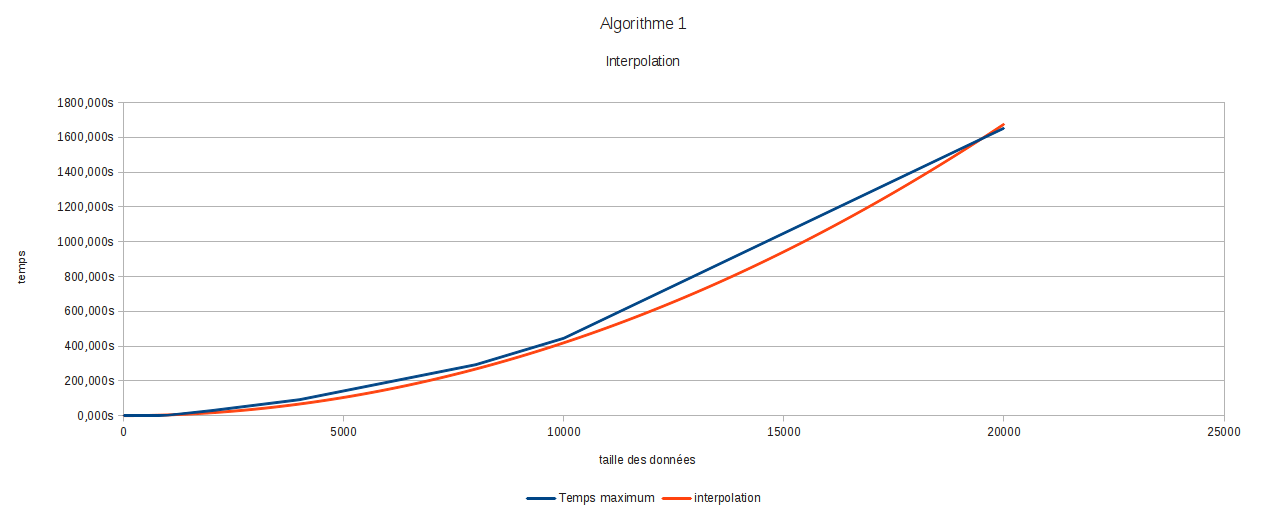
\includegraphics[width=\textwidth]{interpo_algo1}
  \caption{Interpolation de l'algorithme 1}
    \label{interpo1}
\end{figure}
\begin{figure}[p]
  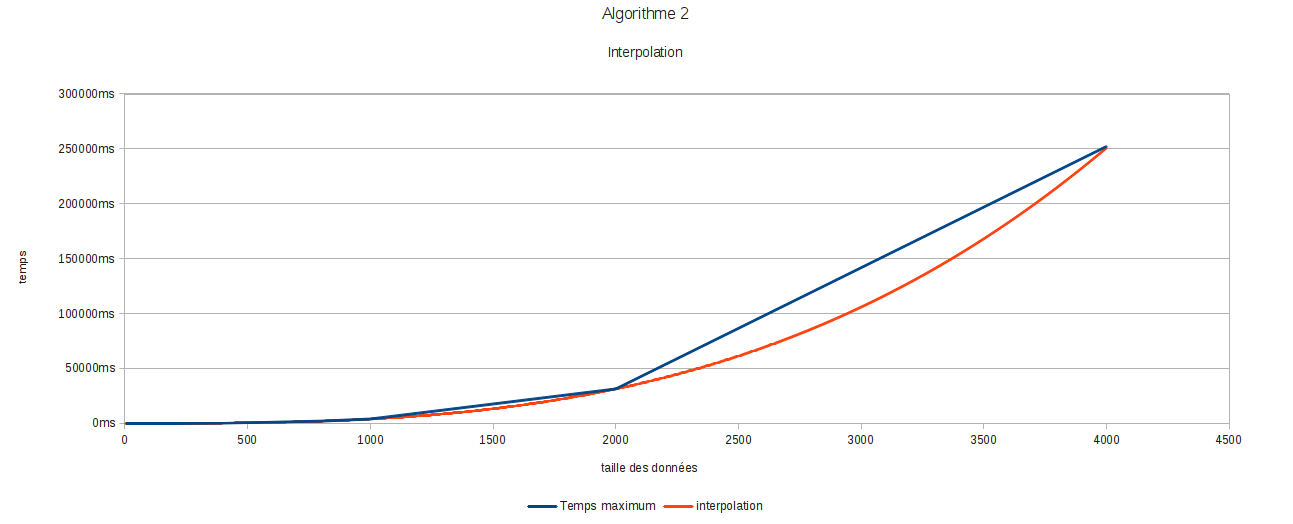
\includegraphics[width=\textwidth]{interpo_algo2}
  \caption{Interpolation de l'algorithme 2}
    \label{interpo2}
\end{figure}
\begin{figure}[p]
  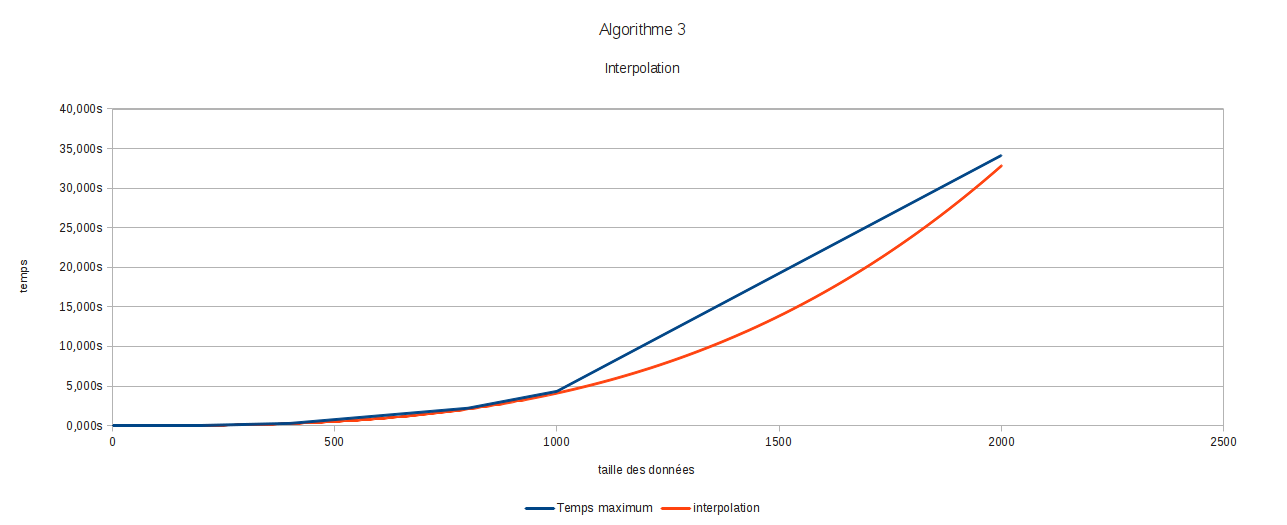
\includegraphics[width=\textwidth]{interpo_algo3}
  \caption{Interpolation de l'algorithme 3}
    \label{interpo3}
\end{figure}

Par la méthode d'approche décrite ci-dessus, nous obtenons pour les trois algorithmes les équations suivantes :
\begin{itemize}
 \item $f_{A_1}(x)=4.09\times 10^{-6} x^2 + 10^{-4}x$ ce qui revient à une complexité en $O(n^2)$ 
 \item $f_{A_2}(x)=3.92\times 10^{-9}x^3 + 10^{-9} x^2 + 5\times 10^{-6} x$ ce qui revient à une complexité en $O(n^3)$ 
  \item $f_{A_3}(x)=4.1\times 10^{-9}x^3 + 10^{-10} x^2 + 3\times 10^{-6} x$ ce qui revient à une complexité en $O(n^3)$ 
\end{itemize}

Les figures \ref{interpo1} \ref{interpo2} et \ref{interpo3} représentent le tracé de la fonction obtenue et leurs comparaison avec la courbe expérimentale de coût au pire pour les trois algorithmes.\\
Les coefficients sont de l'ordre de $10^{-6}$, ce qui s'explique par la puissance actuelle des processeurs, dont la fréquence est de l'ordre de $10^9Hz$. Pour les algorithmes $A_1$ et $A_3$, on retrouve les degrés maximum calculés dans la section \ref{c_theorique}.\\
En revanche, notre ``interpolation'' à partir des résultats de $A_2$ nous donne une fonction en $O(n^3)$ au lieu de $O(n^4)$. Cela peut s'expliquer par un coefficient très faible associé au degré 4 de l'équation réelle. 
Le faible nombre de points dans le tableau nous a permis d'approcher une fonction en $O(n^2)$ probablement invalide pour des valeurs supérieures. De même, l'écart entre la courbe théorique et la courbe extrapolée démontre que notre choix des coefficients n'est pas optimal pour de grandes valeurs.
\part{Conclusion}
\end{document}

